\documentclass{beamer}
\usepackage{beamerthemesplit,graphicx,wrapfig, slashed, subfigure,verbatim,hyperref,color,colortbl,tabularx}
% \usepackage{graphicx,wrapfig, slashed, subfigure,verbatim,hyperref,color,colortbl,tabularx}
\usepackage{amsmath,amssymb}
\usepackage{helvet} %font helvetica
\usepackage{siunitx}
\usepackage{pdftricks}
\usepackage{pstricks}
\usepackage{beamerfoils}
\usepackage{multicol}
%\usepackage{babel}
\usepackage{feynmp-auto}

\usepackage[utf8]{inputenc}
\usepackage[T1]{fontenc}
\usepackage{ulem}
%\usepackage{epstopdf}
\usepackage{color, colortbl}
%\usepackage{biblatex}

% \usetheme{Hannover}
\useoutertheme{infolines2}
%\font\ttfAkkuratLightOffice AkkuratLightOffice-Regular at10pt
\colorlet{structure}{green!50!black}
\definecolor{tugreen}{RGB}{132,184,24}
\definecolor{tugrey}{RGB}{178,179,182}
\definecolor{tured}{RGB}{205,0,47}
\setbeamercolor{palette primary}{bg=tugreen,fg=black}
\setbeamercolor{palette secondary}{bg=tugrey!50!tugreen,fg=black}
\setbeamercolor{palette quaternary}{fg=black, bg=tugrey}
\setbeamercolor{caption name}{fg=tugreen}
\setbeamercolor{palette tertiary}{fg=black,bg=tugrey}


\setbeamercolor{palette compare}{bg=white!80!tugreen,fg=black}
\setbeamercolor{palette misc}{bg=white!80!tugreen,fg=black}
\setbeamercolor{palette white}{bg=white!99!black,fg=black}

\setbeamercolor{itemize item}{fg=tugreen}
\setbeamercolor{itemize subitem}{fg=tugreen}
\setbeamercolor{itemize subsubitem}{fg=tugreen}
\setbeamercolor{enumerate item}{fg=tugreen}
\setbeamertemplate{itemize item}[square]
\setbeamercolor{titlelike}{fg=tugreen, bg=white}
\setbeamertemplate{navigation symbols}{}
\usepackage{tcolorbox}
\definecolor{mycolor}{rgb}{0.122, 0.435, 0.698}% Rule colour
\makeatletter
\newcommand{\mybox}[1]{%
\vspace{1pt}
  \setbox0=\hbox{#1}%
  \setlength{\@tempdima}{\dimexpr\wd0+10pt}%

  \begin{tcolorbox}[colframe=mycolor,boxrule=0.5pt,arc=4pt,
      left=3pt,right=3pt,top=0.5pt,bottom=0pt,boxsep=0pt,width=\@tempdima]
    #1
  \end{tcolorbox}
  \vspace*{-6pt}
}
\makeatother

%%%%%%%%%%%%%%%%%%%%%%%%%%%%%%%%%%%%%%%%%%%%%%%%%%%%%%%%%%%%%%%
\newcommand{\beginbackup}{
   \newcounter{framenumbervorappendix}
   \setcounter{framenumbervorappendix}{\value{framenumber}}

}
  
 \newcommand{\backupend}{
   \addtocounter{framenumbervorappendix}{-\value{framenumber}}
   \addtocounter{framenumber}{\value{framenumbervorappendix}} 
 }
%%%%%%%%%%%%%%%%%%%%%%%%%%%%%%%%%%%%%%%%%%%%%%%%%%%%%%%%%%%%%%%5



\title{CPT Violation in $\phi\rightarrow K^0\overline K^0$}
\subtitle{Can we study it in LHCb?}

\author{Sonja Bartkowski\\
Supervisors: Giulio Dujany \& George Lafferty\\
In collaboration with Lorenzo Capriotti, Jonathan Harrison,\\ Wojciech Krzemien, Jeroen Van Tilburg, \& Wojciech Wislicki\\
\vspace*{-.2cm}}


%\vspace*{-.2cm}
\date{September 1, 2015\\ \vspace{0.5cm}
\vspace*{-.1cm}
\begin{columns}
        \column{.2\textwidth}  \centering 
\includegraphics[width=0.75\textwidth]{TitlePage/AN_cernlogo.pdf}
	\column{.22\textwidth} \centering 
\includegraphics[width=0.8\textwidth]{lhcb_logo.pdf}
	\column{.25\textwidth} \centering 
\includegraphics[width=\textwidth]{UniOfManchesterLogo.pdf}
	        \column{.3\textwidth} \centering 
\includegraphics[width=\textwidth]{TitlePage/tud_logo_cmyk.pdf}
\end{columns}}
\MyLogo{
\includegraphics[width=2.5cm]{lhcb_logo.pdf}} 

\begin{document}

\LogoOff
\frame{\titlepage}

\begin{frame}[fragile]
\frametitle{Who I am}
\vspace*{-.3cm}
\begin{beamercolorbox}[rounded=true,shadow=true]{palette misc}
\vspace*{-.3cm}
\begin{itemize}
\item Master student at the TU Dortmund, Germany
\item Last summer: 
\begin{itemize}
\item Bachelor thesis with ATLAS (top physics)
\item Quantum information processing summer school
\end{itemize}
\item This fall:
\begin{itemize}
\item Start of my master thesis (ATLAS exotics)
\end{itemize}
\item This summer:\\
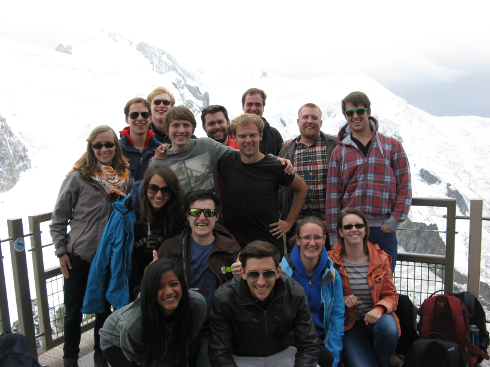
\includegraphics[height = 2.8cm]{Fotos/MB.png}
\hspace{.2cm}
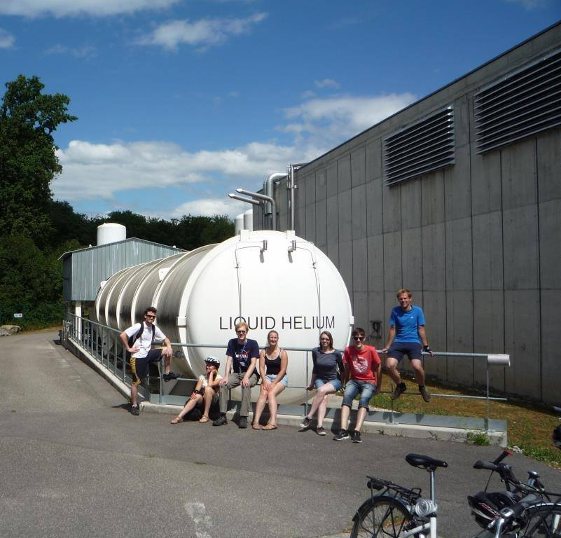
\includegraphics[height = 2.8cm]{Fotos/Bike.png}
\hspace{.2cm}
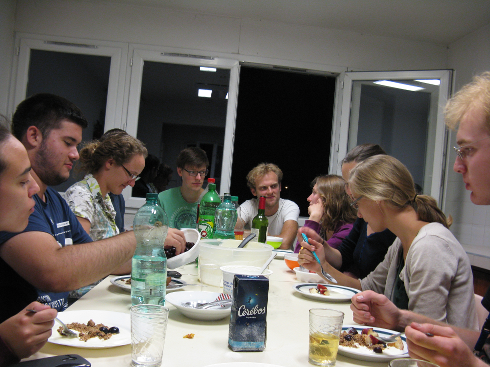
\includegraphics[height = 2.8cm]{Fotos/Lexi.png}
\item And of course the project I am about to show you!
\end{itemize}

\end{beamercolorbox}
\end{frame}

\section{Introduction}


\begin{frame}[fragile]
\frametitle{CPT Violation in neutral kaon systems}

%$\phi \rightarrow K^0 \bar{K}^0$
%
%Because of quantum numbers of $\phi$ $J^{PC} = 1^{--}$,
\begin{equation*}
\left|\phi\right\rangle \rightarrow \frac{1}{\sqrt{2}}\left( \left|K^0\right\rangle \left|\overline K^0\right\rangle - \left|\overline K^0\right\rangle \left|K^0\right\rangle\right)  = \frac{N}{\sqrt{2}} \left(\left|K_S\right\rangle \left| K_L\right\rangle - \left| K_L\right\rangle \left|K_S\right\rangle\right)
\end{equation*}
\begin{itemize}
\item $K_S$ and $K_L$ are not CP eigenstates
\item $K_L \rightarrow \pi^+ \pi^-$ as well as $K_S \rightarrow \pi^+ \pi^-$, $\mathcal{BR}(K_L\rightarrow \pi^+\pi^-) \sim 2\cdot 10^{-3}$
\item Interference in decay intensity:
\end{itemize}
%$K_S = \frac{1}{\sqrt{1+|\epsilon|^2}} \left(\left|K_+\right\rangle + \epsilon \left|K_-\right\rangle\right)$, $K_L = \frac{1}{\sqrt{1+|\epsilon|^2}} \left(\left|K_-\right\rangle + \epsilon \left|K_+\right\rangle\right)$
\Large{
\begin{align*}
I(t_1,t_2) \propto & \color{purple}e^{-\Gamma_L t_1 - \Gamma_S t_2} +e^{-\Gamma_S t_1 - \Gamma_L t_2}\\& \color{black}- 2\color{red}\color{black} e^{-\frac{1}{2}\left(\Gamma_S + \Gamma_L\right)\left(t_1+t_2\right)}\cos\left(\Delta m \left(t_1-t_2\right)\right)
\end{align*}}
\normalsize
\color{white}
Intrinsical violation of CPT introduces decoherence term.


\end{frame}




\begin{frame}[fragile]
\frametitle{CPT Violation in neutral kaon systems}

%$\phi \rightarrow K^0 \bar{K}^0$
%
%Because of quantum numbers of $\phi$ $J^{PC} = 1^{--}$,
\begin{equation*}
\left|\phi\right\rangle \rightarrow \frac{1}{\sqrt{2}}\left( \left|K^0\right\rangle \left|\overline K^0\right\rangle - \left|\overline K^0\right\rangle \left|K^0\right\rangle\right)  = \frac{N}{\sqrt{2}} \left(\left|K_S\right\rangle \left| K_L\right\rangle - \left| K_L\right\rangle \left|K_S\right\rangle\right)
\end{equation*}
\begin{itemize}
\item $K_S$ and $K_L$ are not CP eigenstates
\item $K_L \rightarrow \pi^+ \pi^-$ as well as $K_S \rightarrow \pi^+ \pi^-$, $\mathcal{BR}(K_L\rightarrow \pi^+\pi^-) \sim 2\cdot 10^{-3}$
\item Interference in decay intensity:
\end{itemize}
%$K_S = \frac{1}{\sqrt{1+|\epsilon|^2}} \left(\left|K_+\right\rangle + \epsilon \left|K_-\right\rangle\right)$, $K_L = \frac{1}{\sqrt{1+|\epsilon|^2}} \left(\left|K_-\right\rangle + \epsilon \left|K_+\right\rangle\right)$
\Large{
\begin{align*}
I(t_1,t_2) \propto & e^{-\Gamma_L t_1 - \Gamma_S t_2} +e^{-\Gamma_S t_1 - \Gamma_L t_2}\\& \color{purple}- 2 e^{-\frac{1}{2}\left(\Gamma_S + \Gamma_L\right)\left(t_1+t_2\right)}\cos\left(\Delta m \left(t_1-t_2\right)\right)
\end{align*}}
\normalsize
\color{white}
Intrinsical violation of CPT introduces decoherence term.

\setcounter{framenumber}{3} 
\end{frame}




\begin{frame}[fragile]
\frametitle{CPT Violation in neutral kaon systems}

%$\phi \rightarrow K^0 \bar{K}^0$
%
%Because of quantum numbers of $\phi$ $J^{PC} = 1^{--}$,
\begin{equation*}
\left|\phi\right\rangle \rightarrow \frac{1}{\sqrt{2}}\left( \left|K^0\right\rangle \left|\overline K^0\right\rangle - \left|\overline K^0\right\rangle \left|K^0\right\rangle\right)  = \frac{N}{\sqrt{2}} \left(\left|K_S\right\rangle \left| K_L\right\rangle - \left| K_L\right\rangle \left|K_S\right\rangle\right)
\end{equation*}
\begin{itemize}
\item $K_S$ and $K_L$ are not CP eigenstates
\item $K_L \rightarrow \pi^+ \pi^-$ as well as $K_S \rightarrow \pi^+ \pi^-$, $\mathcal{BR}(K_L\rightarrow \pi^+\pi^-) \sim 2\cdot 10^{-3}$
\item Interference in decay intensity:
\end{itemize}
%$K_S = \frac{1}{\sqrt{1+|\epsilon|^2}} \left(\left|K_+\right\rangle + \epsilon \left|K_-\right\rangle\right)$, $K_L = \frac{1}{\sqrt{1+|\epsilon|^2}} \left(\left|K_-\right\rangle + \epsilon \left|K_+\right\rangle\right)$
\Large{
\begin{align*}
I(t_1,t_2) \propto & e^{-\Gamma_L t_1 - \Gamma_S t_2} +e^{-\Gamma_S t_1 - \Gamma_L t_2}\\& - 2\color{red}(1-\zeta_{SL})\color{black} e^{-\frac{1}{2}\left(\Gamma_S + \Gamma_L\right)\left(t_1+t_2\right)}\cos\left(\Delta m \left(t_1-t_2\right)\right)
\end{align*}}
\normalsize
Intrinsical violation of CPT introduces decoherence term.

\setcounter{framenumber}{3} 
\end{frame}



\begin{frame}[fragile]
\frametitle{CPT Violation in neutral kaon systems}
\vspace*{-.2cm}
Intrinsical violation of CPT introduces decoherence term.\footnote{There are different decoherence models, but we will stick with this one for now for the sake of simplicity.}
\vspace*{-.2cm}
\large{
\begin{align*}
I(t_1,t_2) \propto & e^{-\Gamma_L t_1 - \Gamma_S t_2} +e^{-\Gamma_S t_1 - \Gamma_L t_2}\\& - 2(1-\zeta_{SL}) e^{-\frac{1}{2}\left(\Gamma_S + \Gamma_L\right)\left(t_1+t_2\right)}\cos\left(\Delta m \left(t_1-t_2\right)\right)
\end{align*}}
\normalsize
\vspace*{-.3cm}
\begin{columns}
\begin{column}{.49\columnwidth}
\tiny{$I(\Delta t)$[a.u.]}\vspace*{-.3cm}
\begin{center}
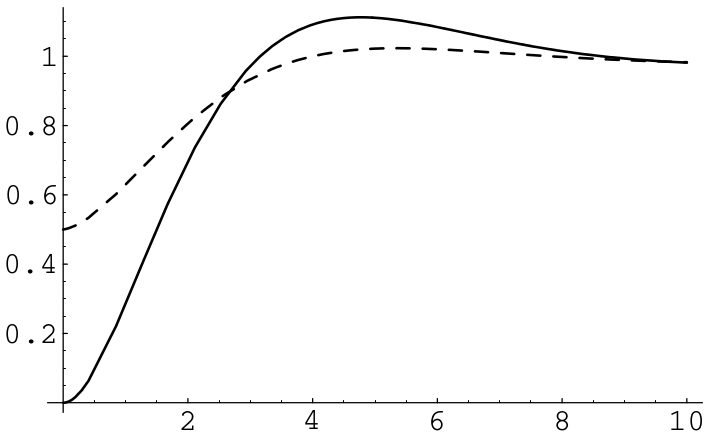
\includegraphics[width = .9\columnwidth]{Excess.png}
\end{center}
\flushright{\vspace*{-.4cm}$\Delta t/\tau_S$}

\vspace{.1cm}
\tiny{[CPT and Quantum Mechanics Tests with Kaons,\\ J. Bernabeu et al., \href{http://arxiv.org/abs/hep-ph/0607322}{arXiv:hep-ph/0607322}]}
\end{column}

\normalsize

\begin{column}{.49\columnwidth}
\centering
$\Rightarrow$ Excess of 4$\pi$ decays \\for small $\Delta t$
\end{column}

\end{columns}

\end{frame}
\section{Comparison}
\begin{frame}[fragile]
\frametitle{Comparison of two approaches}
\vspace*{-.2cm}
\begin{columns}
\begin{column}{.49\columnwidth}
\centering{\underline{Prompt $\mathbf{\phi}$}}
\begin{itemize}
\item high production cross section
\end{itemize}
\vspace{1.1cm}
\centering
\begin{fmffile}{incl}
		\setlength{\unitlength}{.5mm}
		\fmfframe(0,0)(10,10){
		\begin{fmfgraph*}(75,65)
			\fmfleft{l1}
			\fmfright{r1,r2,r3,r4}
			\fmflabel{$\pi^+$}{r1}
			\fmflabel{$\pi^-$}{r2}					
			\fmflabel{$\pi^+$}{r3}
			\fmflabel{$\pi^-$}{r4}
			\fmf{plain}{r1,x1,r2}
			\fmf{plain}{r3,x2,r4}
			\fmf{dashes,label=$K_L$}{x1,y1}
			\fmf{dashes,label=$K_S$}{y1,x2}
			\fmf{dashes,label=$\phi$}{l1,y1}
			\fmfforce{(.2w,.5h)}{y1}
		\end{fmfgraph*}}
\end{fmffile}
\vspace{.2cm}
\end{column}
\begin{column}{.49\columnwidth}
\centering{\underline{$D_S^\pm\rightarrow \mathbf{\phi}\pi^\pm$}}
\begin{itemize}
\item lower rate ($\sim$1\%)
\item possibly better handle on background rejection
\end{itemize}
\vspace{.4cm}
\centering
\begin{fmffile}{Ds}
		\setlength{\unitlength}{.5mm}
		\fmfframe(0,0)(10,10){
		\begin{fmfgraph*}(75,65)
			\fmfleft{l1}
			\fmfright{r1,r2,r3,r4,r5}
			\fmflabel{$\pi^+$}{r1}
			\fmflabel{$\pi^-$}{r2}					
			\fmflabel{$\pi^+$}{r3}
			\fmflabel{$\pi^-$}{r4}
			\fmf{plain}{r1,x1,r2}
			\fmf{plain}{r3,x2,r4}
			\fmf{dashes,label=$K_L$}{x1,y1}
			\fmf{dashes,label=$K_S$}{y1,x2}
			\fmf{dashes,label=$\phi$}{z1,y1}
			\fmf{plain}{l1,z1}
			\fmf{plain}{z1,r5}
			\fmflabel{$D_S^\pm$}{l1}
			\fmflabel{$\pi^\pm$}{r5}
		\end{fmfgraph*}}
\end{fmffile}

\end{column}

\end{columns}

\begin{itemize}
\item First study on the prompt $\phi$ approach
\item Compare with $D_S$ approach
\end{itemize}

\end{frame}
\section{Terminology}
\begin{frame}
\frametitle{Terminology}
\begin{columns}
\begin{column}{.4\columnwidth}
$\frac{}{}$
\end{column}
\begin{column}{.6\columnwidth}
\begin{itemize}
\item[Signal: ] Excess of $\phi \rightarrow $ 2 neutral kaons $ \rightarrow \pi^+\pi^-\pi^+\pi^-$ for $\Delta t$ small due to CPT violation
\item[SM background: ] Resulting from CPV, $\phi \rightarrow K_L K_S \rightarrow \pi^+\pi^-\pi^+\pi^-$
\item[Regeneration background: ] Regeneration $K_L \rightarrow K_S$ in material\
\item[Combinatoric background: ] Prompt kaons and pions

\end{itemize}
\end{column}
\end{columns}






\end{frame}


\section{Selection}
\begin{frame}
\frametitle{Selection}

\begin{itemize}
\item Stripping for the prompt $\phi$ approach already existed
\end{itemize}

\centering
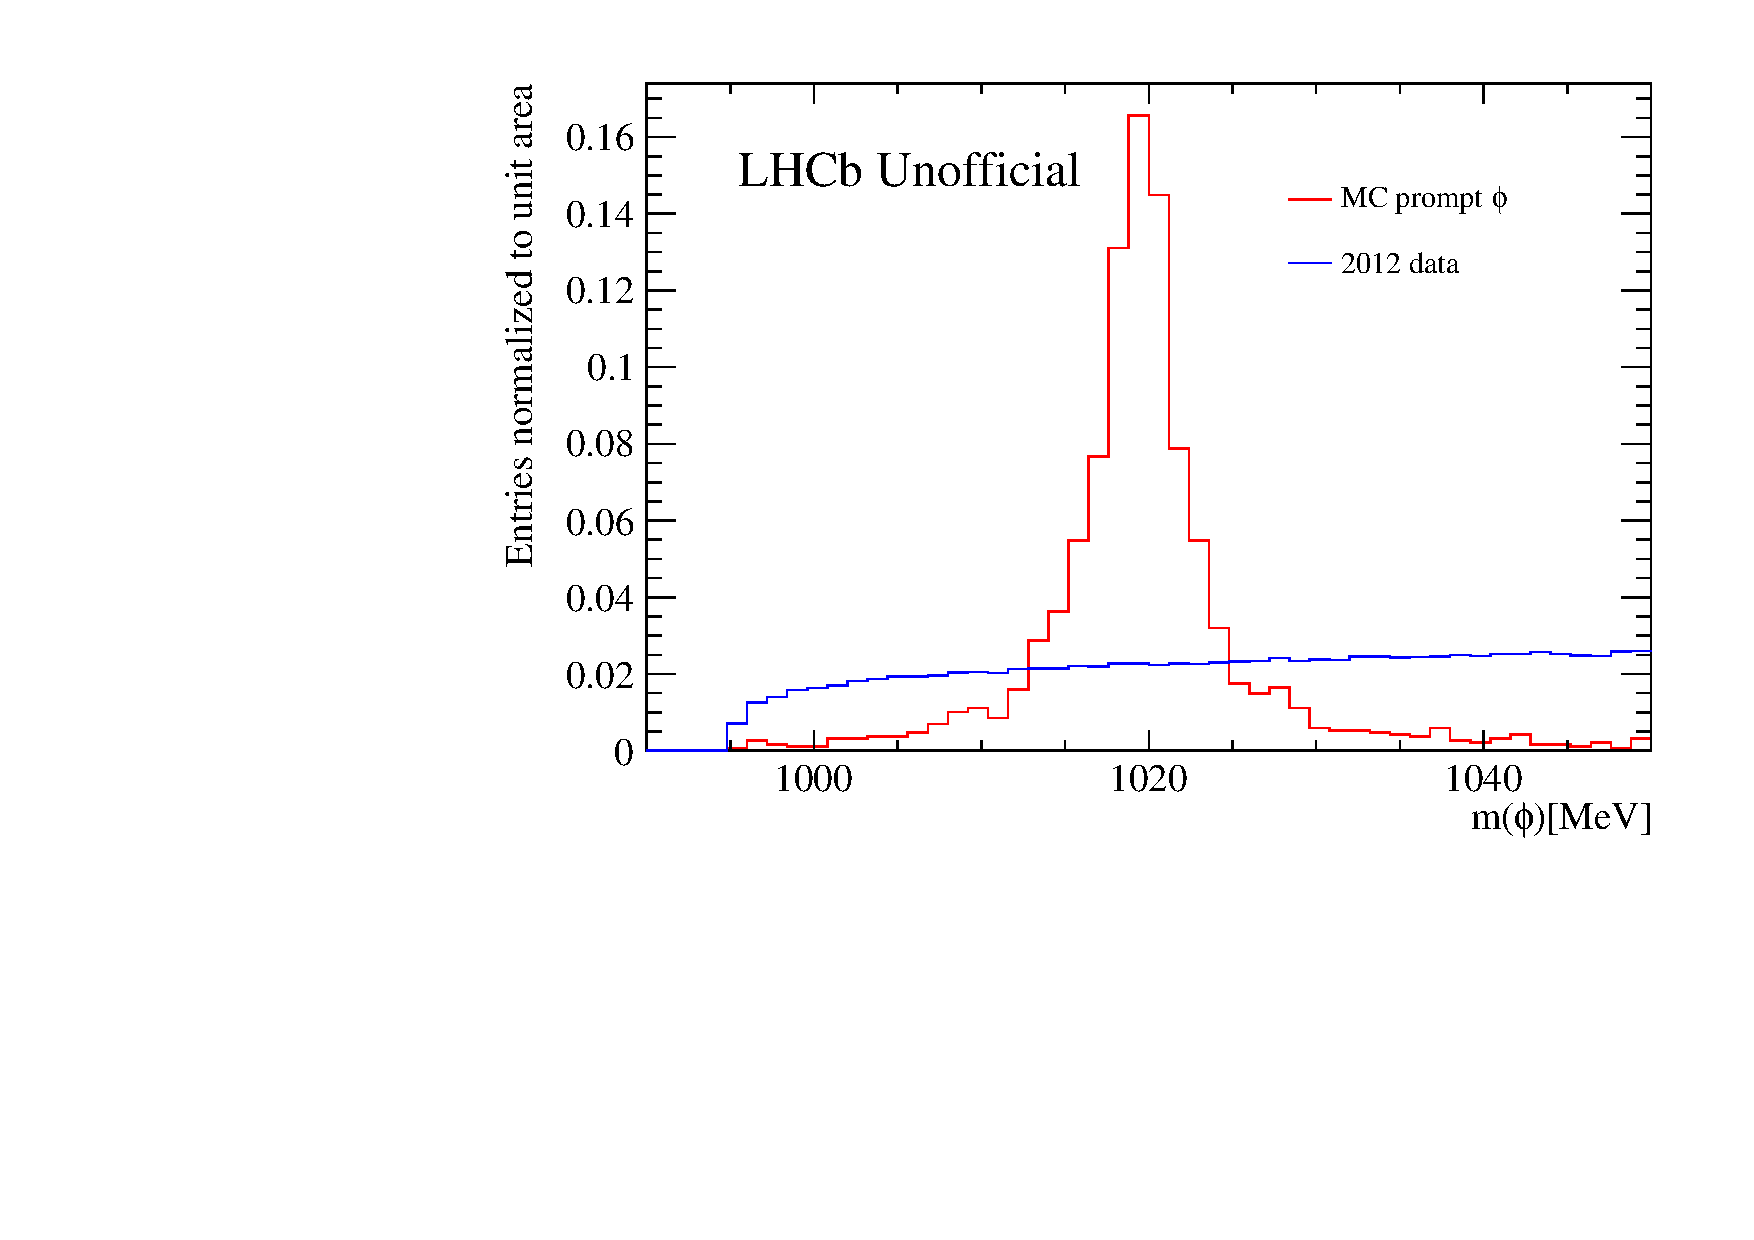
\includegraphics[width = .85\columnwidth]{/home/soonja/lxplus/phi2KsKs/phi2KsKs/preliminaryStudies/m_phi_incl.pdf}

\end{frame}


\begin{frame}
\frametitle{Selection}

\begin{itemize}
\item Developed selection for $D_S \rightarrow \phi \pi$
\begin{itemize}
\item Cuts on the mass regions of $\phi$ and $D_S$
\item Cuts on the $\chi^2$ of the impact parameter of  $\phi$\\ to exclude prompt $\phi$
\end{itemize}
\end{itemize}
\vspace*{-.2cm}
\begin{columns}
\begin{column}{.5\columnwidth}
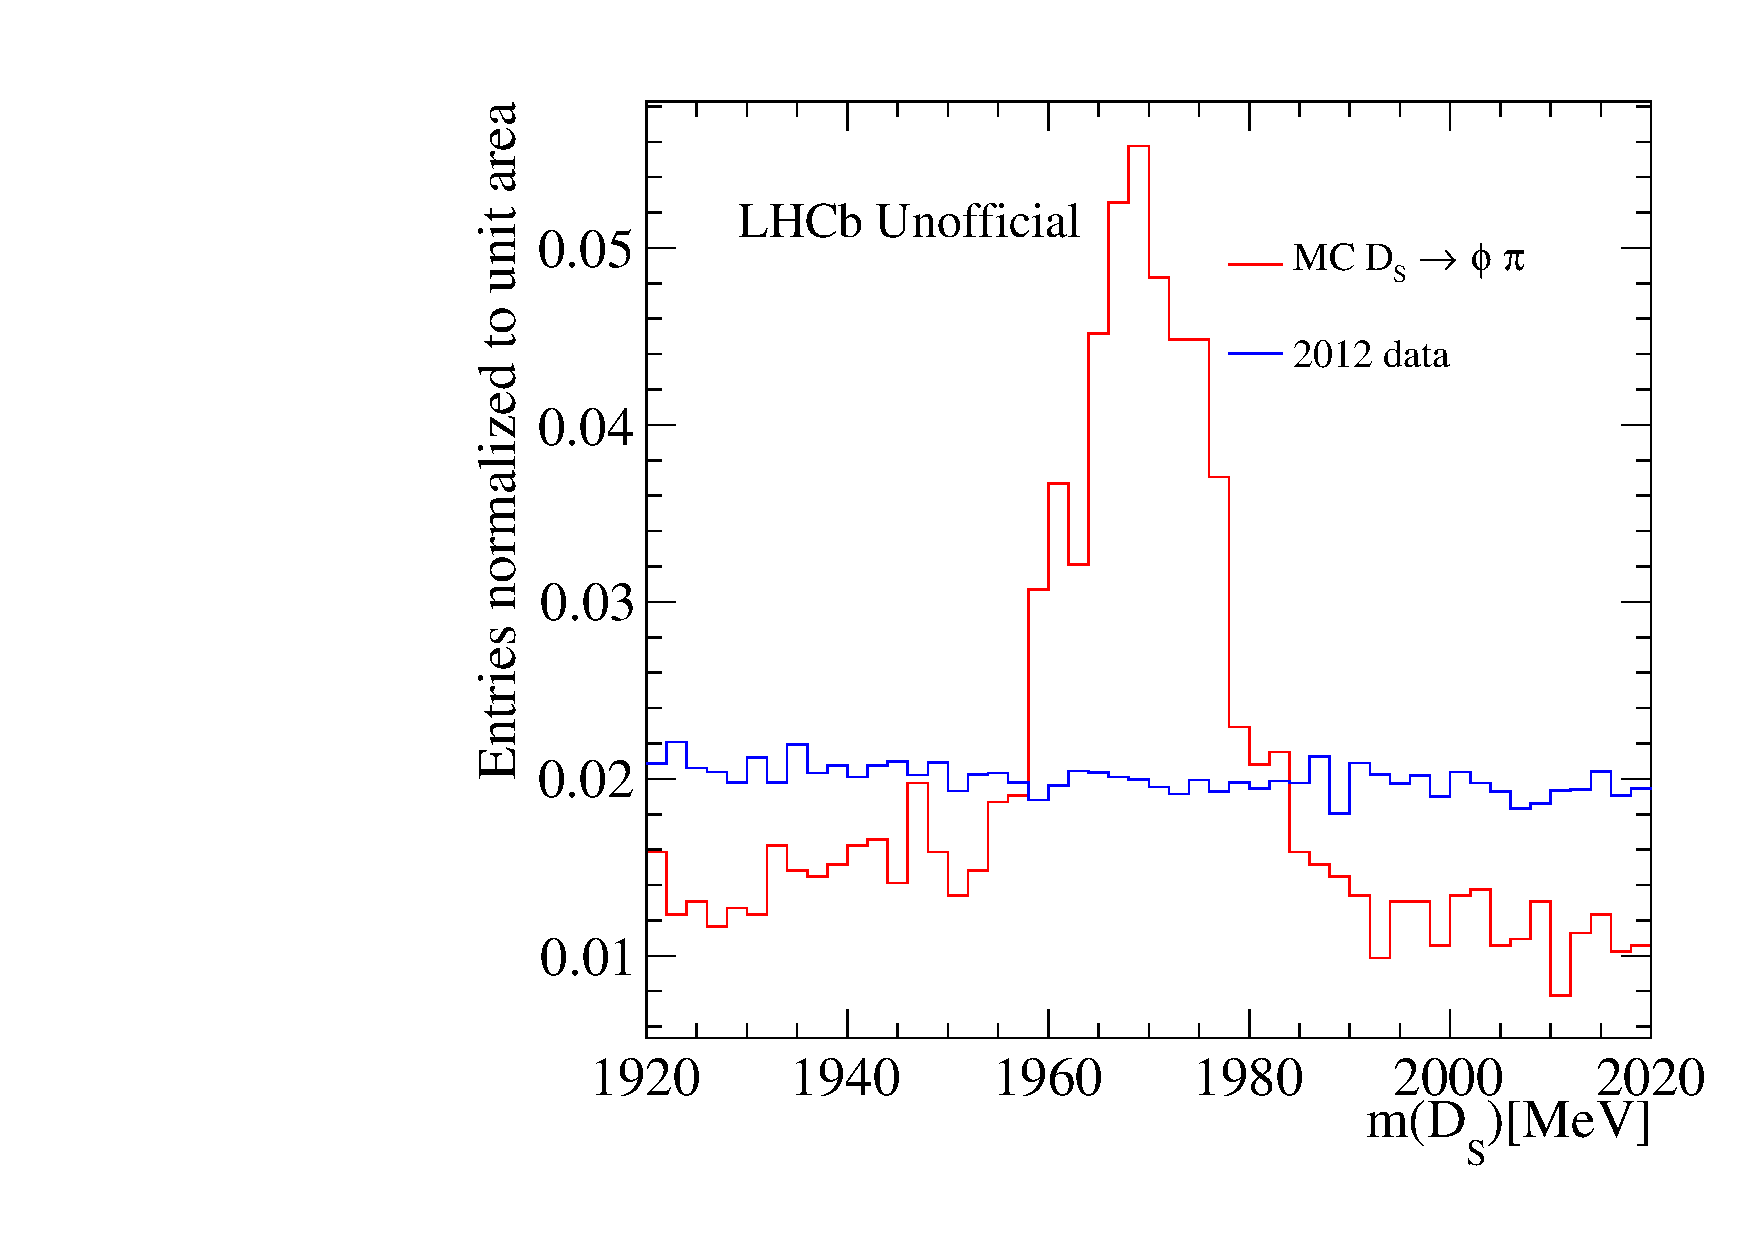
\includegraphics[width = \columnwidth]{/home/soonja/lxplus/phi2KsKs/phi2KsKs/preliminaryStudies/m_Ds_Ds.pdf}
\end{column}
\begin{column}{.5\columnwidth}
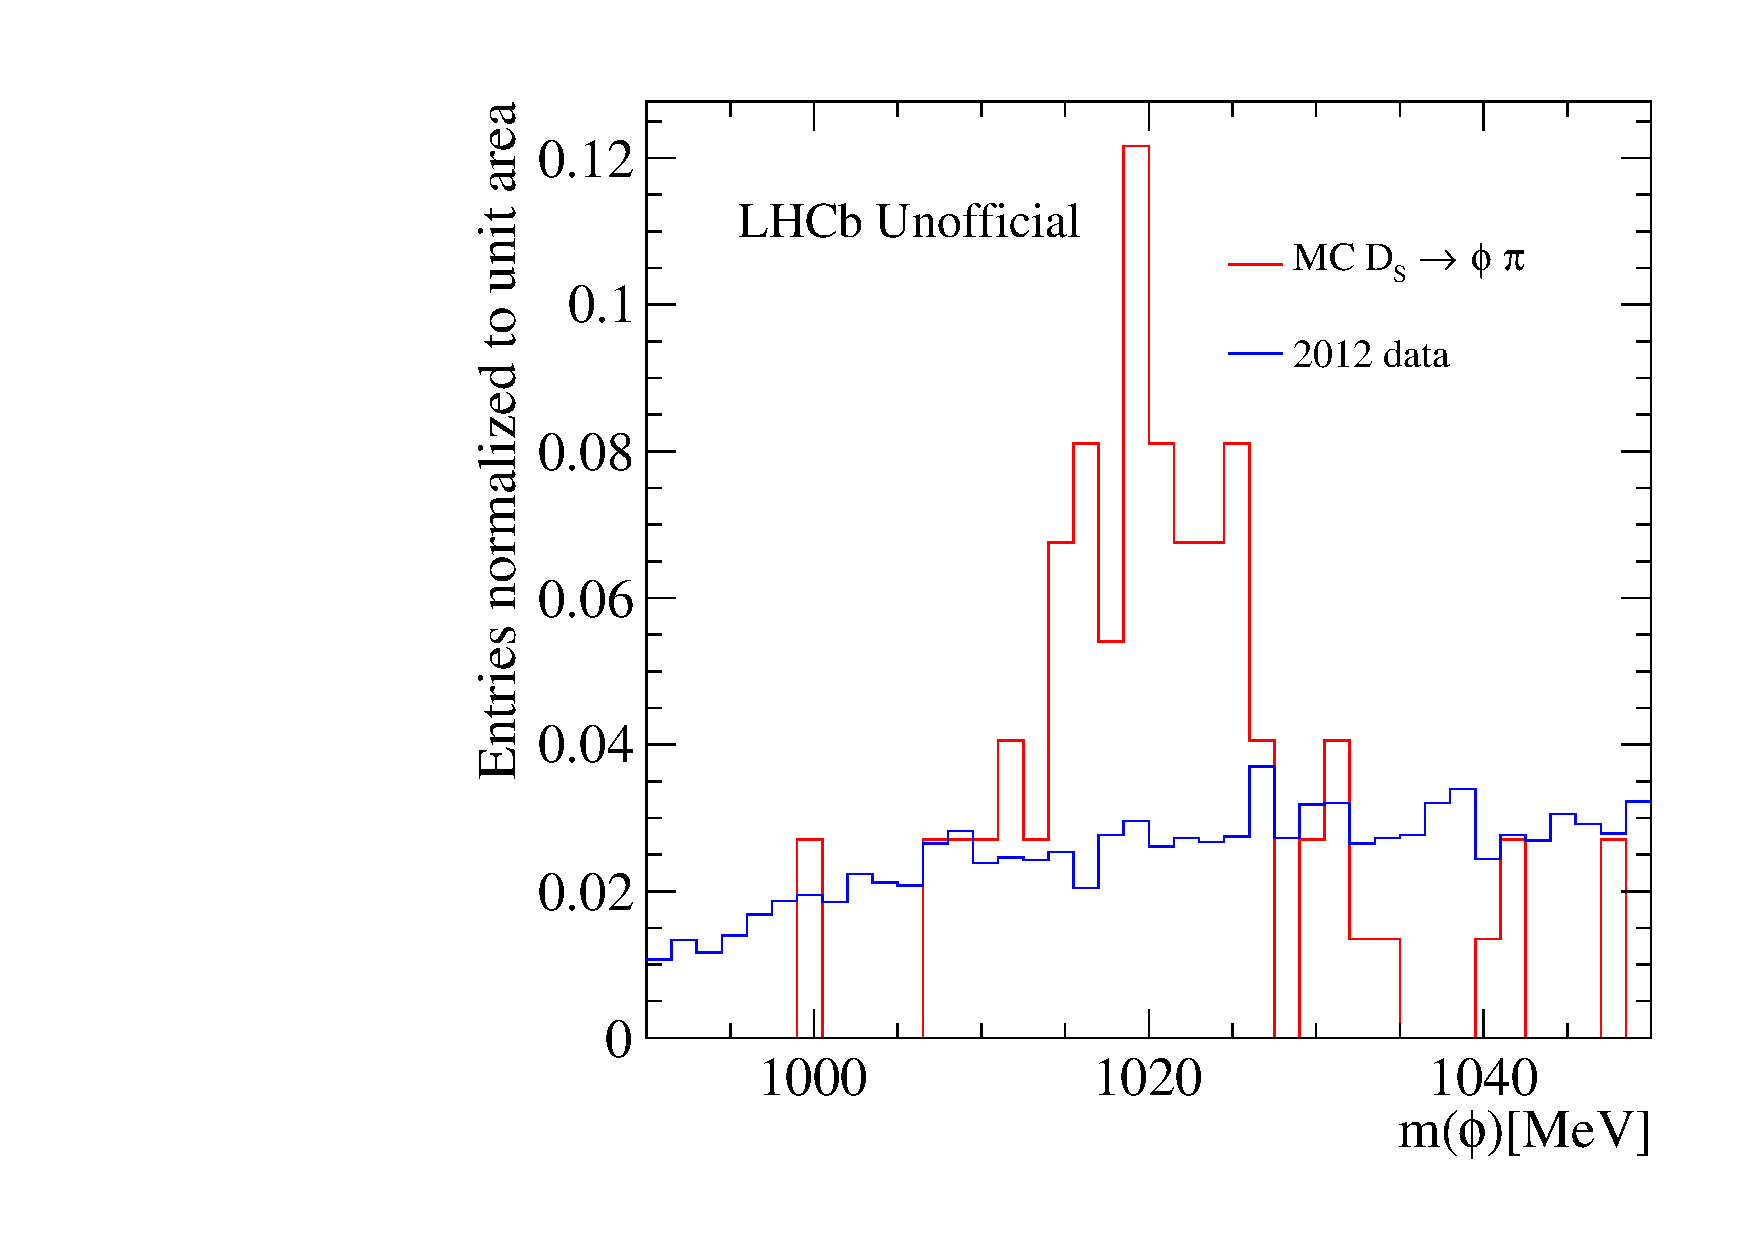
\includegraphics[width = \columnwidth]{/home/soonja/lxplus/phi2KsKs/phi2KsKs/preliminaryStudies/m_phi_Ds.pdf}
\end{column}
\end{columns}
\end{frame}




\begin{frame}
\frametitle{Efficiencies}
\begin{scriptsize}
\resizebox{\textwidth}{!}{
\begin{tabular}{ccc}
&Prompt $\phi$ & $D_s \rightarrow \phi \pi$ \\
\hline 
\hline
\vspace*{-6pt}\\
Cross section (\SI{14}{TeV}), LHCb acceptance &\mybox{\SI{ 3516 }{\micro\barn}} & \mybox{\SI{ 388 }{\micro\barn}} \\
\hline
\vspace*{-6pt}\\
Branching fractions & \mybox{34.2\%} & \mybox{4.5\% $\cdot$  34.2\% }\\
\hline
\vspace*{-7pt}\\
Fiducial cuts efficiency & 2.5\% & 7.0\%\\
\hline
Prob. $K_sK_s \rightarrow 4\pi$, \\
 exactly 1 (2) decays inside bp &\multicolumn{2}{c}{$ 15.1\%$ ( $2.8\%$ )} \\
\hline
Prob. $K_sK_L \rightarrow 4\pi$ (CPV),\\
exactly 1 (2) decays inside bp &\multicolumn{2}{c}{$ 3.98\cdot 10^{-7}$ ( $4.99\cdot 10^{-10}$ )} \\
\hline
Upper limit KLOE prob. $K_sK_L \rightarrow 4\pi$ (CPV \\
+ CPTV), exactly 1 (2) decays inside bp &\multicolumn{2}{c}{$  5.13\cdot 10^{-7}$ ( $1.64\cdot 10^{-8}$ )}\\
\hline
\vspace{-8pt}\\
Reconstruction \& selection efficiency &  7.9\% ( 7.6\% )  & 1.4\% ( 4.2\%)\\
\hline
\vspace{-8pt}\\
L0 efficiency&  16.1\% ( 18.6\% )&  22.4\% ( 18.2\% )\\
LT1 efficiency&  13.7\% ( 16.7\% )& 45.5\% ( 25.0\% )\\
HLT2 efficiency&  65.6\% ( 100.0\% )& 75.0\% ( 100.0\% )\\
\hline
\hline
\vspace{-8pt}\\
Total efficiency SM background &$ 4.39\cdot 10^{-5}$ ( $5.85\cdot 10^{-5}$ )&$ 1.02\cdot 10^{-4}$ ( $1.32\cdot 10^{-4}$ )\\
Expected events SM background / fb$^{-1}$ &\mybox{$21$ ( $3.51\cdot 10^{-2}$ )}& \mybox{$2.43\cdot 10^{-1}$ ( $3.94\cdot 10^{-4}$ )}\\
\vspace{-10pt}\\
Upper limit for signal (KLOE) & $27$ ( $1.15$ )&  $3.13\cdot 10^{-1}$ ( $ 1.29\cdot 10^{-2}$ )\\
Background (data 2012) / fb$^{-1}$ & \mybox{163110 ( 29120 )} &  \mybox{1170 ( 6100 )}\\
\end{tabular}
}
\end{scriptsize}
\end{frame}

\begin{frame}
\frametitle{Efficiencies new}
\begin{scriptsize}
\resizebox{\textwidth}{!}{
\begin{tabular}{ccc}
&Prompt $\phi$ & $D_s \rightarrow \phi \pi$ \\
\hline 
Cross section (\SI{14}{TeV}), LHCb acceptance & \SI{ 3516 }{\micro\barn} & \SI{ 388 }{\micro\barn} \\
Branching fractions & 34.2 \% & 4.5  \% $\cdot$  34.2 \% \\
Generator cut efficiency & 2.5 \% & 7.0 \%\\
Probability of $K_sK_L \rightarrow 4\pi$ with exactly 1 (2) decays in the beam pipe  with limit on decoherence of KLOE&\multicolumn{2}{c}{$  5.13\cdot 10^{-7} $($ 1.64\cdot 10^{-8} $)} \\
Probability of $K_sK_L \rightarrow 4\pi$ with exactly 1 (2) decays in the beam pipe &\multicolumn{2}{c}{$ 3.98\cdot 10^{-7} $($ 4.99\cdot 10^{-10} $)} \\
Probability of $K_sK_s \rightarrow 4\pi$ with exactly 1 (2) decays in the beam pipe &\multicolumn{2}{c}{$ 15.1 \% $($ 2.8 \% $)} \\
Reconstruction \& selection efficiency &  7.9 \%( 7.6 \%)  & 1.4 \%( 3.9 \%)\\
L0 efficiency&  16.1 \%( 18.6 \%)&  23.0 \%( 19.5 \%)\\
HLT1 efficiency&  13.7 \%( 16.7 \%)& 35.6 \%( 25.0 \%)\\
HLT2 efficiency&  65.6 \%( 100.0 \%)& 68.8 \%( 100.0 \%)\\
\hline
Total efficiency SM background &$ 4.39\cdot 10^{-5} $($ 5.85\cdot 10^{-5} $)&$ 8.18\cdot 10^{-5} $($ 1.32\cdot 10^{-4} $)\\
Expected events SM background / fb$^{-1}$ &$ 21 $($ 3.51\cdot 10^{-2} $)&$ 1.94\cdot 10^{-1} $($ 3.94\cdot 10^{-4} $)\\
Upper limit for signal (KLOE) &$ 27 $($ 1.15 $)&$ 2.5\cdot 10^{-1} $($ 1.29\cdot 10^{-2} $)\\
Background (data 2012) / fb$^{-1}$ & 163110 ( 29120 ) &  450 ( 2030 )\\
\end{tabular}
}
\end{scriptsize}
\end{frame}








\begin{frame}
\frametitle{Efficiencies}
Conclusion:
\begin{itemize}
\item Background dominates over signal for both approaches
\item For the $D_S$ approach, both signal and background rate go down by two orders of magnitude compared to the prompt $\phi$ approach
\begin{itemize}
\item There is no big improvement in the signal to background ratio
\end{itemize}
\end{itemize}

\end{frame}







\section{Feasibility study}





\LogoOff
\begin{frame}[fragile]
\frametitle{Feasibility study for prompt $\phi$}

Studies of minimum bias Monte Carlo suggest that \\80\% background is prompt $K_S$
\begin{itemize}
\item this background is irreducible
\item $I(t_1,t_2) \propto e^{-\Gamma_St_1} \,e^{-\Gamma_St_2}$
\end{itemize}
\vspace*{6pt}
Toy study with RooFit!
\begin{itemize}
\item decay intensity
\item momentum distribution
\item 1 kaon decaying inside beampipe
\item regeneration not taken into account
\end{itemize}
\vspace*{6pt}
But first: Studying resolution for toy study
\end{frame}

\begin{frame}
\frametitle{Time resolution}
\vspace*{-4mm}
\begin{center}
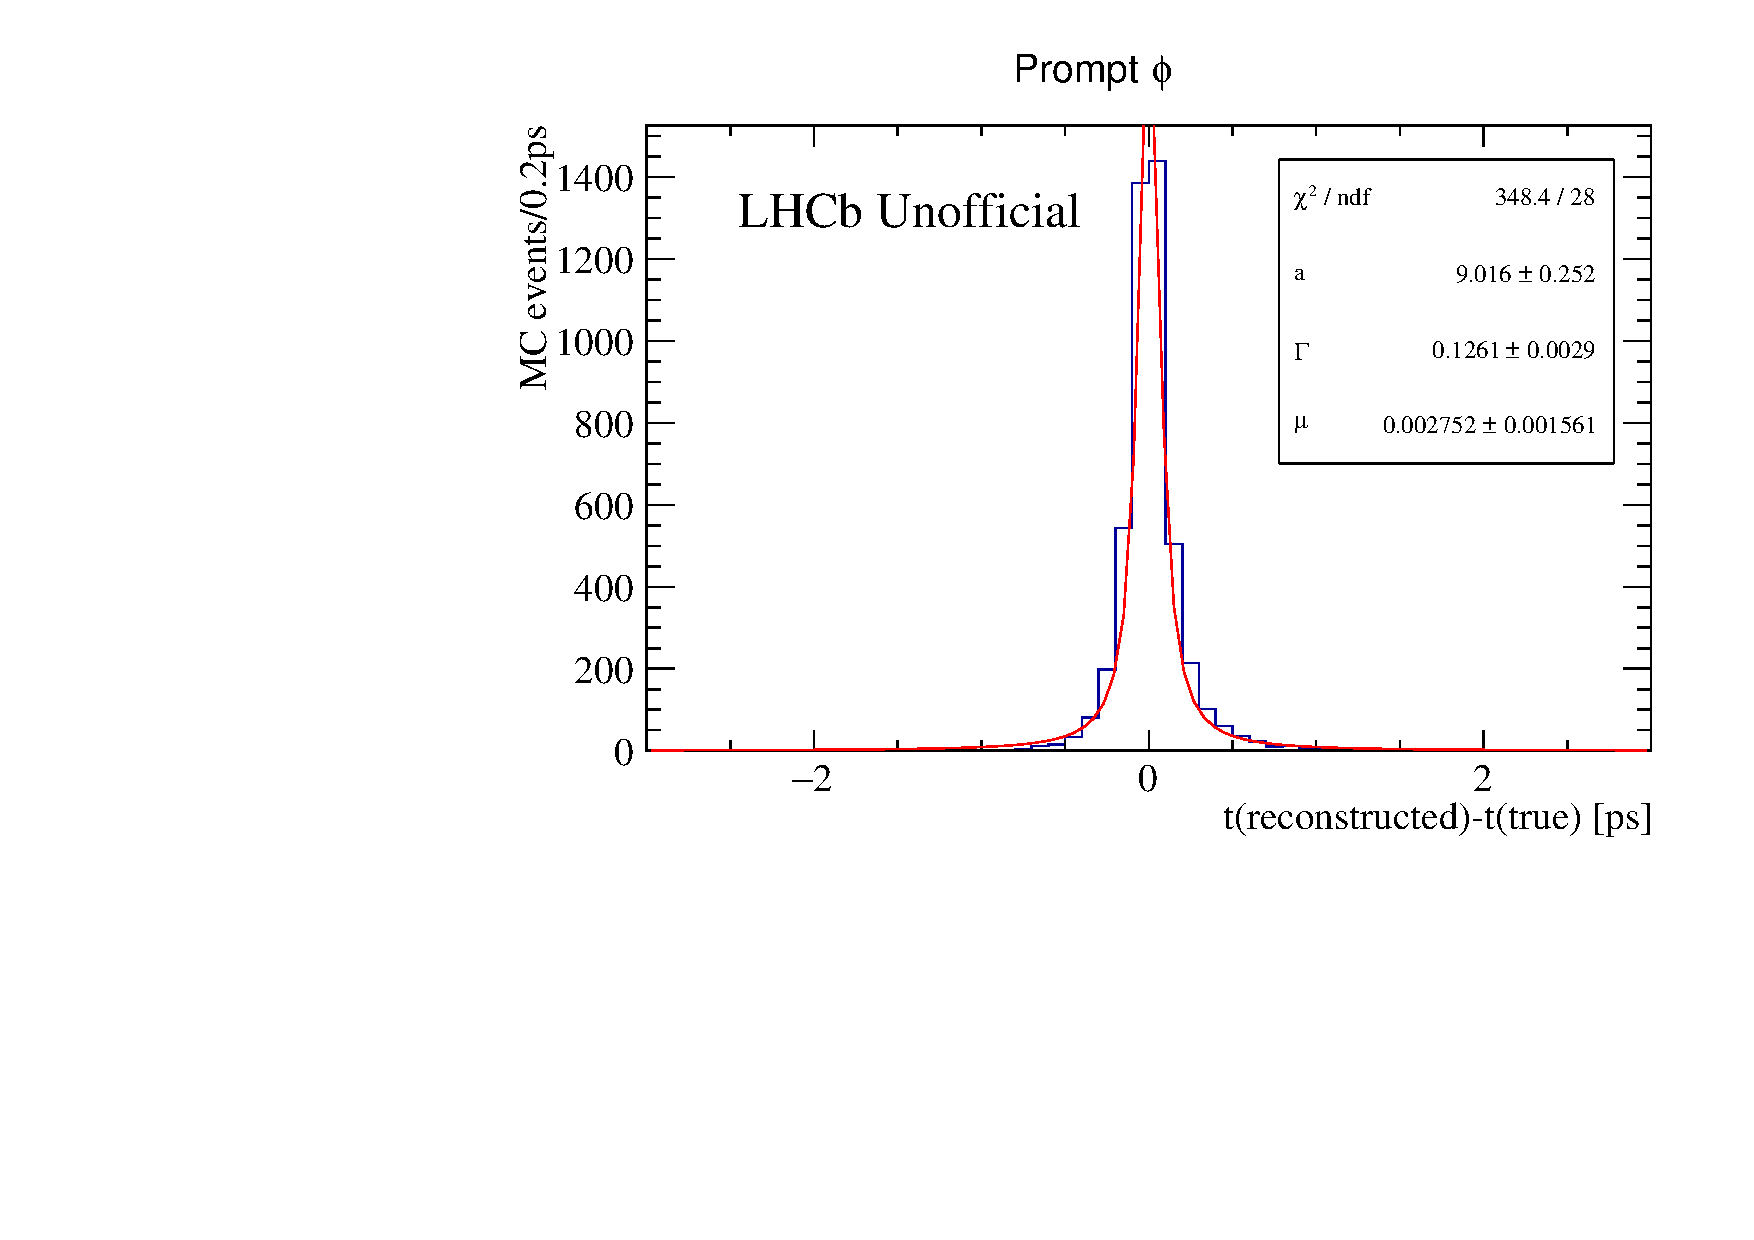
\includegraphics[width=.85\textwidth]{/home/soonja/lxplus/phi2KsKs/phi2KsKs/preliminaryStudies/timeResolution-LL.pdf}
\end{center}
\vspace*{-4mm}
Resolution of the core of the distribution is a few ps\\
$\Rightarrow$ 5 ps binning in toy study
\end{frame}


\begin{frame}[fragile]
\frametitle{Feasibility study for prompt $\phi$}

\begin{columns}
\begin{column}{.5\textwidth}
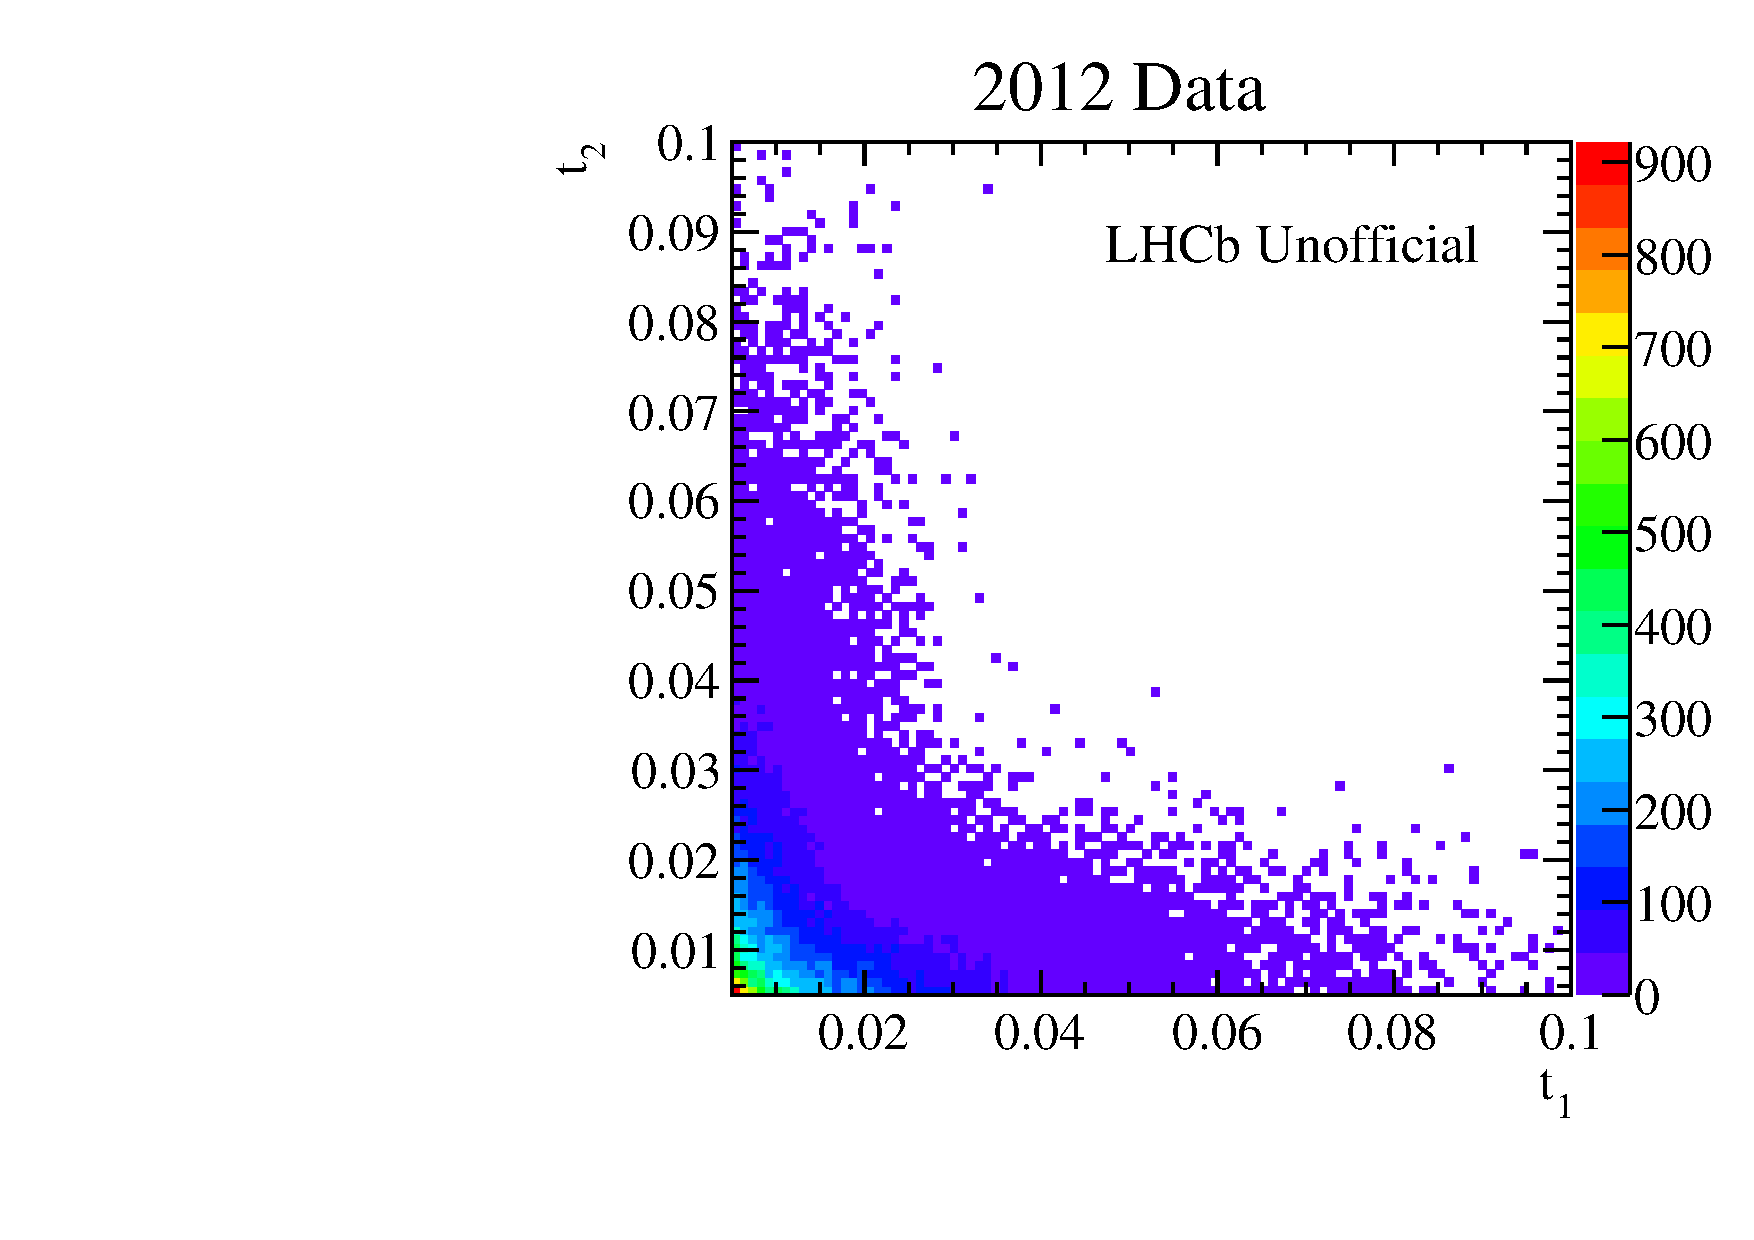
\includegraphics[width =\columnwidth,trim= 0mm 0mm 0mm 0mm, clip]{/home/soonja/lxplus/phi2KsKs/phi2KsKs/toymodell/data.pdf}
\end{column}

\begin{column}{.5\textwidth}
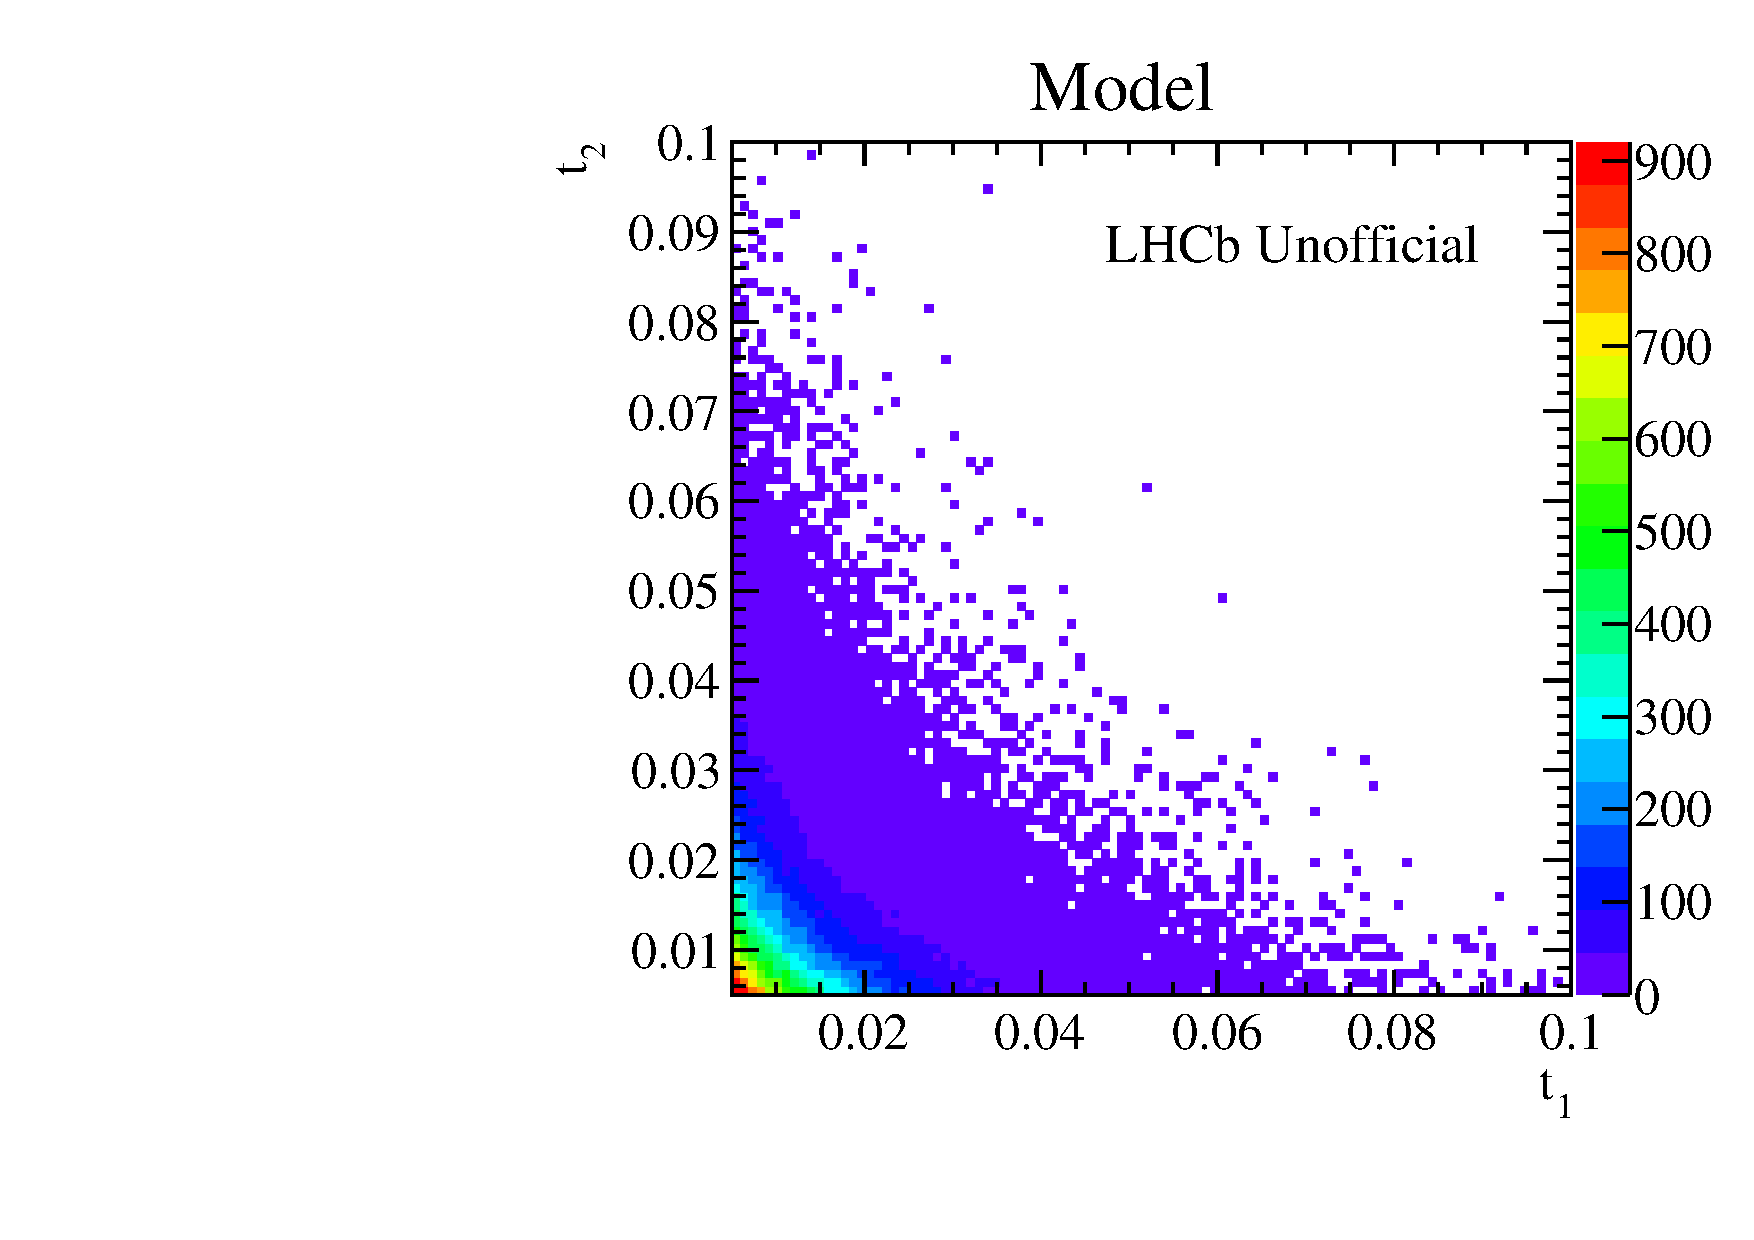
\includegraphics[width =\columnwidth]{/home/soonja/lxplus/phi2KsKs/phi2KsKs/toymodell/model.pdf}
\end{column}
\end{columns}

\end{frame}

\begin{frame}
\frametitle{Feasibility study for prompt $\phi$}
\begin{itemize}
\item Using optimistic signal to background ratio of $4\cdot 10^{-4}$
\item RooStats profile likelihood calculator
\item Fitted with square root of luminosity
\end{itemize}

\begin{columns}
\begin{column}{.7\columnwidth}
\vspace*{-.3cm}
\begin{center}
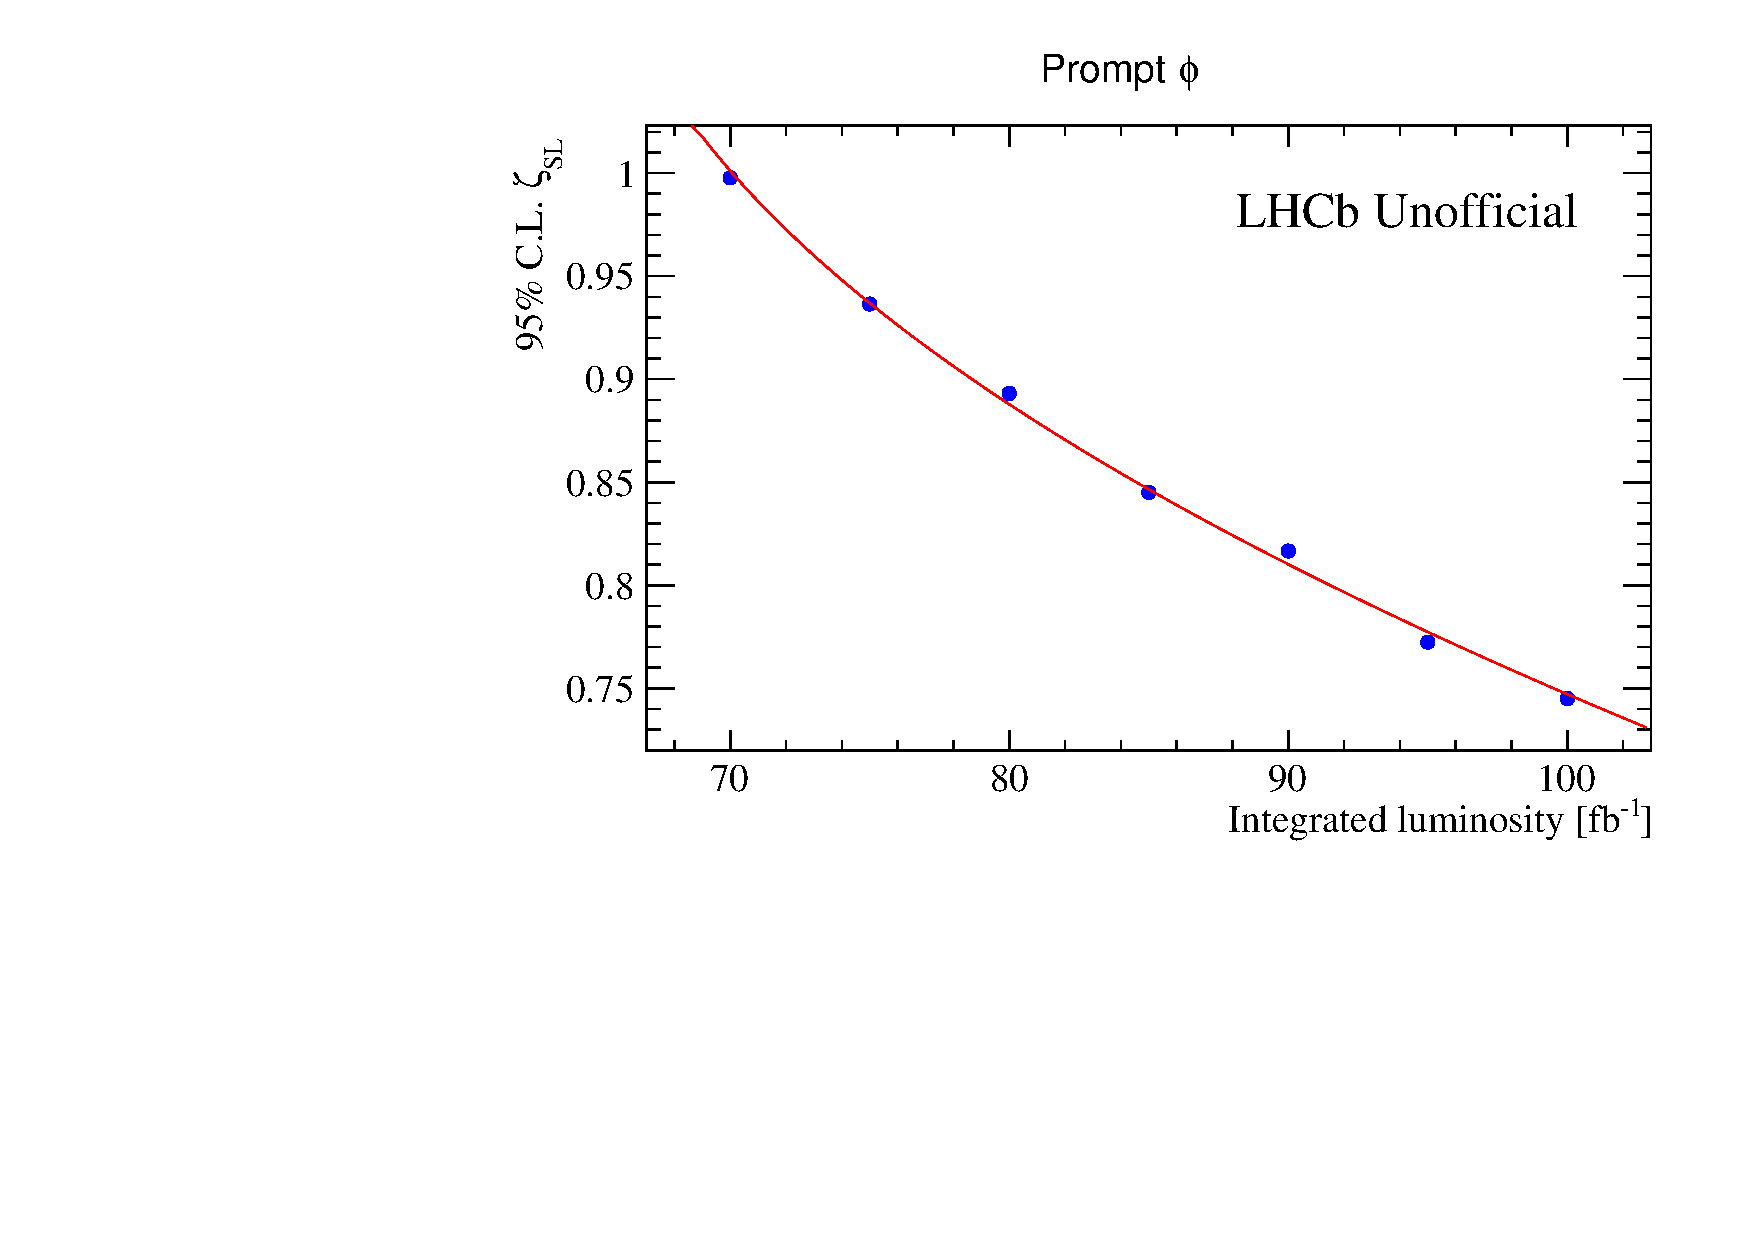
\includegraphics[width=\columnwidth,trim= 0mm 0mm 0mm 10mm, clip]{/home/soonja/lxplus/phi2KsKs/phi2KsKs/toymodell/limits.pdf}

\end{center}
\end{column}
\begin{column}{.29\columnwidth}\centering
For KLOE limit $\zeta_{SL} = 0.098$\\
$\Downarrow$\\
$\int L \;dt \approx 275$ fb$^{-1}$,
extrapolated\\ from fit
\end{column}
\end{columns}
\end{frame}


\begin{frame}[fragile]
\frametitle{Summary}

\begin{beamercolorbox}[rounded=true,shadow=true]{palette misc}

\begin{itemize}
\item Selection for $D_S \rightarrow \phi \pi$ implemented
\item Compared the prompt $\phi$ and the $D_S$ approach
\begin{itemize}
\item For both strategies, the background dominates.
\end{itemize}
\item The time resolution is a few ps
\item Performed a toy study for the prompt $\phi$ approach\\ to estimate limits we can set on CPTV
\end{itemize}
After my studies, the prospects for this analysis look bleak.
\end{beamercolorbox}
\pause
\vspace{.8cm}
\hspace{1cm}\huge\color{tugreen}{Thank you for your attention!}
\end{frame}
% \LogoOn





\section{Backup}
%--------------------BACKUP--------------------------------------
\beginbackup

\begin{frame}
  \begin{block}{\color{tugreen}\Huge \bfseries \center BACKUP\color{black}}
  \end{block}
\end{frame}


\begin{frame}
\frametitle{Toy study}
\begin{itemize}
\item Generated toy data as the weighted sum of two distributions in decay times:
\begin{itemize}
\item[1.] Combinatoric background of prompt $K_S$ with decay intensity
\begin{equation*}
I(t_1,t_2) \propto e^{-\Gamma_S t_1}e^{-\Gamma_S t_2}  
\end{equation*}
\item[2.] SM background with decay intensity
\begin{align*}
I(t_1,t_2) \propto & e^{-\Gamma_L t_1 - \Gamma_S t_2} +e^{-\Gamma_S t_1 - \Gamma_L t_2}\\& - 2 e^{-\frac{1}{2}\left(\Gamma_S + \Gamma_L\right)\left(t_1+t_2\right)}\cos\left(\Delta m \left(t_1-t_2\right)\right)
\end{align*}
\end{itemize}
\item Ratio of SM background to combinatoric background from efficiency study
\item Fitted to 
\begin{align*}
I(t_1,t_2) \propto & e^{-\Gamma_L t_1 - \Gamma_S t_2} +e^{-\Gamma_S t_1 - \Gamma_L t_2}\\& - 2(1-\zeta_{SL}) e^{-\frac{1}{2}\left(\Gamma_S + \Gamma_L\right)\left(t_1+t_2\right)}\cos\left(\Delta m \left(t_1-t_2\right)\right)
\end{align*}
\item Derived limit on $\zeta_{SL}$ from fit result 
\end{itemize}
\end{frame}




\LogoOff
\begin{frame}[fragile]
\frametitle{Selection - prompt $\phi$}

\begin{beamercolorbox}[rounded=true,shadow=true]{palette misc}
\centering{Prompt $\phi$ production}
\begin{itemize}
\item Stripping PhiToKSKS\_PhiToKsKsLine
\begin{itemize}
\item[$\pi$] 
TRGHOSTPROB < 0.35\\
P $>$ 2.GeV\\
MIPCHI2DV(PRIMARY) $>$ 9.\\
\item[$K_S$]ADMASS('KS0') < 35.MeV\\
VFASPF(VCHI2) < 25.\\
\item[$\phi$]LL or LD combinations $^{*)}$\\
APT > 400 MeV\\
VFASPF(VCHI2/VDOF) < 6\\
MIPCHI2DV(PRIMARY) < 9\\
M < 1100 MeV\\
\end{itemize}
\item $\SI{1010}{MeV}<$phi\_M$<\SI{1030}{MeV}$
\end{itemize}
\end{beamercolorbox}
$^{*)}$ because of regeneration, KLOE follows the same approach



\end{frame}
\LogoOn

\LogoOff
\begin{frame}[fragile]
\frametitle{Selection - $D_s \rightarrow \phi \pi$}
\vspace*{-2mm}
\begin{beamercolorbox}[rounded=true,shadow=true]{palette misc}
\vspace*{-3mm}
\begin{itemize}
\item Selection (inspired by PhiToKSKS\_PhiToKsKsLine and other charm lines) on CHARMCOMPLETEEVENT.DST

\begin{columns}
\begin{column}{.01\textwidth}
$\frac{}{}$
\end{column}
\begin{column}{.46\textwidth}
\vspace*{-.3mm}
\begin{itemize}
\item[$\pi$($K_S$)]
PT $>$ 150 MeV\\
BPVIPCHI2() $>$ 1.0\\
TRCHI2DOF $<$ 5\\
TRGHOSTPROB $<$ 0.3\\
\item[$K_S$] ADMASS('KS0') $<$ 35 MeV\\
VFASPF(VCHI2) $<$ 2.\\
PT $>$ 200 MeV\\
BPVVD $>$ 10.0 mm\\
BPVVDCHI2 $>$ 100\\
VFASPF(VCHI2PDOF) $<$ 10\\
BPVDIRA $>$ 0.999\\
\end{itemize}


\end{column}
\begin{column}{.48\textwidth}
\begin{itemize}
\item[$\phi$]LL or LD combinations\\
ADMASS('phi(1020)')$<$70 MeV\\
VFASPF(VCHI2/VDOF) $<$ 6\\
APT $>$ 400 MeV\\
\item[$\pi$($D_S$)]TRGHOSTPROB $<$ 0.35\\
P $>$ 2 GeV\\
MIPCHI2DV(PRIMARY) $>$ 9 \\
\item[$D_S$]ADMASS('D\_s+') $<$ 150MeV\\
(BPVVDCHI2 $>$ 16.0) or (BPVLTIME() $>$ 0.150 ps)\\
VFASPF(VCHI2/VDOF) $<$ 25.0\\
\end{itemize}

\end{column}
\end{columns}

\item \SI{1010}{MeV}$<$phi\_M$<$\SI{1030}{MeV} \& \SI{1955}{MeV}$<$Ds\_M$<$\SI{1985}{MeV}
\item IPCHI2 $\geq$ 15,\small{ (possible to tighten cut if more MC statistics available)}
\end{itemize}
\end{beamercolorbox}




\end{frame}


\begin{frame}[fragile]
\frametitle{Backgrounds}
Estimates from minimum bias MC (42 M events). The number in brackets is the number of background events with physical $K_s$.
\begin{center}
\begin{tabular}{c|c|c}
Background category & prompt $\phi$ & $D_s \rightarrow \phi \pi$ \\ 
\hline 
light flavour & 17(17) & 0 \\ 
$b\overline{b}$ & 1(1) & 0 \\ 
different PV & 3(2) & 0 \\ 
physical bkg, partl. reconstructed & 1(1) & 1(1) \\ 
ghosts & 0 & 1(0) \\ 
\hline 
total & 21(20) & 2(1) \\  
\end{tabular} 
\end{center}
Remaining background for prompt $\phi$ is mostly irreducible.

\end{frame}

\begin{frame}[fragile]
\frametitle{Terminology}

\begin{center}
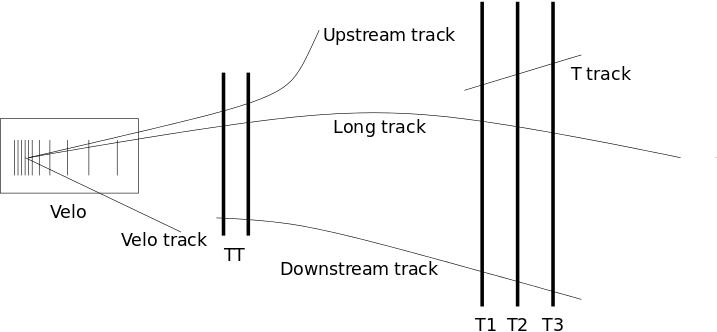
\includegraphics[width = 0.9\textwidth]{tracktypes.png}
\end{center}
\end{frame}

\begin{frame}[fragile]
\frametitle{Time resolution}

\begin{center}
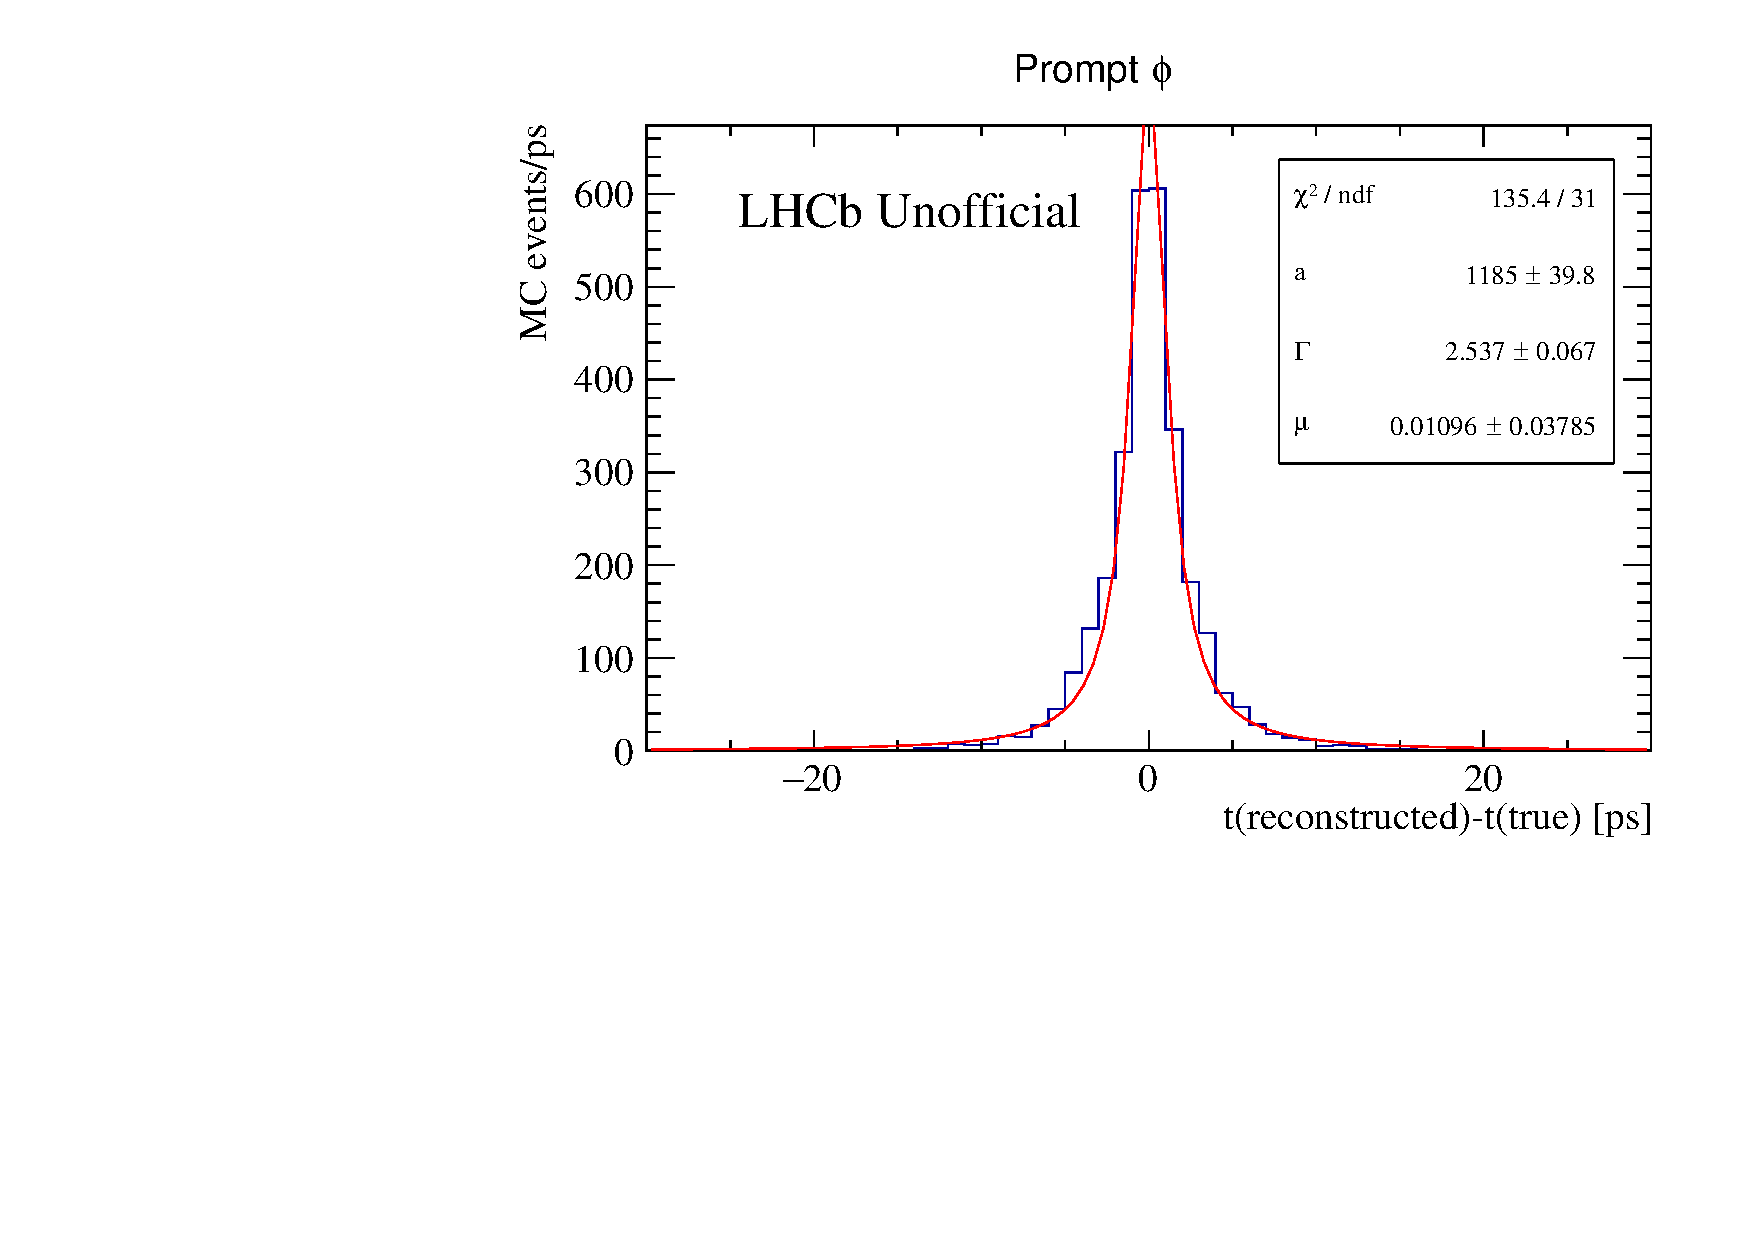
\includegraphics[width=.85\textwidth]{/home/soonja/lxplus/phi2KsKs/phi2KsKs/preliminaryStudies/timeResolution-DD.pdf}
\end{center}

\end{frame}

\backupend
\end{document}